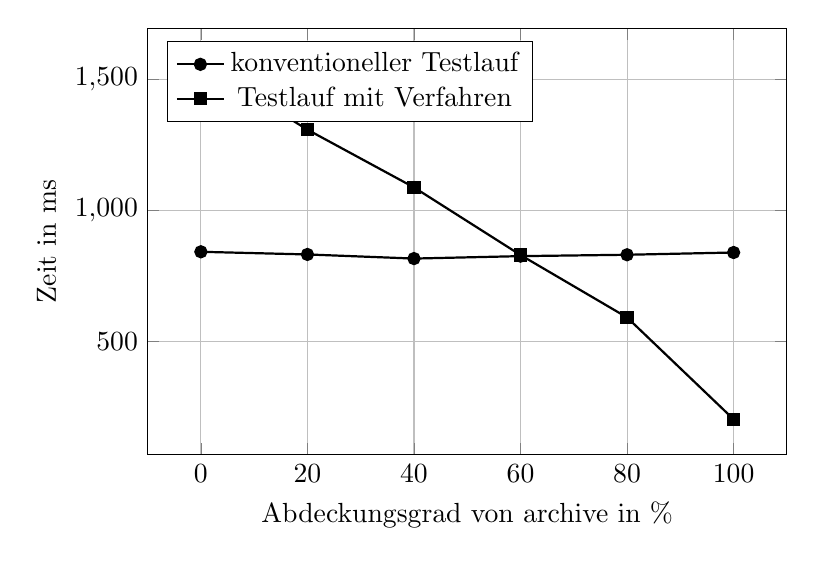
\begin{tikzpicture}
    \begin{axis}[
        width=0.8\textwidth,
        height=7cm,
        xlabel={Abdeckungsgrad von archive in \%},
        ylabel={Zeit in ms},
        grid=major,
        legend pos=north west
    ]
    \addplot[
        thick,
        mark=*,
    ] coordinates {
        (0, 841.5)
        (20, 831.4)
        (40, 815.7)
        (60, 825.0)
        (80, 830.2)
        (100, 838.8)
    };
    \addlegendentry{konventioneller Testlauf}
    \addplot[
        thick,
        mark=square*,
    ] coordinates {
        (0, 1558.4)
        (20, 1307.2)
        (40, 1087.1)
        (60, 829.2)
        (80, 591.2)
        (100, 202.8)
    };
    \addlegendentry{Testlauf mit Verfahren}
    \end{axis}
\end{tikzpicture}
